% Options for packages loaded elsewhere
\PassOptionsToPackage{unicode}{hyperref}
\PassOptionsToPackage{hyphens}{url}
%
\documentclass[
]{article}
\usepackage{amsmath,amssymb}
\usepackage{lmodern}
\usepackage{ifxetex,ifluatex}
\ifnum 0\ifxetex 1\fi\ifluatex 1\fi=0 % if pdftex
  \usepackage[T1]{fontenc}
  \usepackage[utf8]{inputenc}
  \usepackage{textcomp} % provide euro and other symbols
\else % if luatex or xetex
  \usepackage{unicode-math}
  \defaultfontfeatures{Scale=MatchLowercase}
  \defaultfontfeatures[\rmfamily]{Ligatures=TeX,Scale=1}
\fi
% Use upquote if available, for straight quotes in verbatim environments
\IfFileExists{upquote.sty}{\usepackage{upquote}}{}
\IfFileExists{microtype.sty}{% use microtype if available
  \usepackage[]{microtype}
  \UseMicrotypeSet[protrusion]{basicmath} % disable protrusion for tt fonts
}{}
\makeatletter
\@ifundefined{KOMAClassName}{% if non-KOMA class
  \IfFileExists{parskip.sty}{%
    \usepackage{parskip}
  }{% else
    \setlength{\parindent}{0pt}
    \setlength{\parskip}{6pt plus 2pt minus 1pt}}
}{% if KOMA class
  \KOMAoptions{parskip=half}}
\makeatother
\usepackage{xcolor}
\IfFileExists{xurl.sty}{\usepackage{xurl}}{} % add URL line breaks if available
\IfFileExists{bookmark.sty}{\usepackage{bookmark}}{\usepackage{hyperref}}
\hypersetup{
  pdftitle={Statistik},
  hidelinks,
  pdfcreator={LaTeX via pandoc}}
\urlstyle{same} % disable monospaced font for URLs
\usepackage[margin=1in]{geometry}
\usepackage{color}
\usepackage{fancyvrb}
\newcommand{\VerbBar}{|}
\newcommand{\VERB}{\Verb[commandchars=\\\{\}]}
\DefineVerbatimEnvironment{Highlighting}{Verbatim}{commandchars=\\\{\}}
% Add ',fontsize=\small' for more characters per line
\usepackage{framed}
\definecolor{shadecolor}{RGB}{248,248,248}
\newenvironment{Shaded}{\begin{snugshade}}{\end{snugshade}}
\newcommand{\AlertTok}[1]{\textcolor[rgb]{0.94,0.16,0.16}{#1}}
\newcommand{\AnnotationTok}[1]{\textcolor[rgb]{0.56,0.35,0.01}{\textbf{\textit{#1}}}}
\newcommand{\AttributeTok}[1]{\textcolor[rgb]{0.77,0.63,0.00}{#1}}
\newcommand{\BaseNTok}[1]{\textcolor[rgb]{0.00,0.00,0.81}{#1}}
\newcommand{\BuiltInTok}[1]{#1}
\newcommand{\CharTok}[1]{\textcolor[rgb]{0.31,0.60,0.02}{#1}}
\newcommand{\CommentTok}[1]{\textcolor[rgb]{0.56,0.35,0.01}{\textit{#1}}}
\newcommand{\CommentVarTok}[1]{\textcolor[rgb]{0.56,0.35,0.01}{\textbf{\textit{#1}}}}
\newcommand{\ConstantTok}[1]{\textcolor[rgb]{0.00,0.00,0.00}{#1}}
\newcommand{\ControlFlowTok}[1]{\textcolor[rgb]{0.13,0.29,0.53}{\textbf{#1}}}
\newcommand{\DataTypeTok}[1]{\textcolor[rgb]{0.13,0.29,0.53}{#1}}
\newcommand{\DecValTok}[1]{\textcolor[rgb]{0.00,0.00,0.81}{#1}}
\newcommand{\DocumentationTok}[1]{\textcolor[rgb]{0.56,0.35,0.01}{\textbf{\textit{#1}}}}
\newcommand{\ErrorTok}[1]{\textcolor[rgb]{0.64,0.00,0.00}{\textbf{#1}}}
\newcommand{\ExtensionTok}[1]{#1}
\newcommand{\FloatTok}[1]{\textcolor[rgb]{0.00,0.00,0.81}{#1}}
\newcommand{\FunctionTok}[1]{\textcolor[rgb]{0.00,0.00,0.00}{#1}}
\newcommand{\ImportTok}[1]{#1}
\newcommand{\InformationTok}[1]{\textcolor[rgb]{0.56,0.35,0.01}{\textbf{\textit{#1}}}}
\newcommand{\KeywordTok}[1]{\textcolor[rgb]{0.13,0.29,0.53}{\textbf{#1}}}
\newcommand{\NormalTok}[1]{#1}
\newcommand{\OperatorTok}[1]{\textcolor[rgb]{0.81,0.36,0.00}{\textbf{#1}}}
\newcommand{\OtherTok}[1]{\textcolor[rgb]{0.56,0.35,0.01}{#1}}
\newcommand{\PreprocessorTok}[1]{\textcolor[rgb]{0.56,0.35,0.01}{\textit{#1}}}
\newcommand{\RegionMarkerTok}[1]{#1}
\newcommand{\SpecialCharTok}[1]{\textcolor[rgb]{0.00,0.00,0.00}{#1}}
\newcommand{\SpecialStringTok}[1]{\textcolor[rgb]{0.31,0.60,0.02}{#1}}
\newcommand{\StringTok}[1]{\textcolor[rgb]{0.31,0.60,0.02}{#1}}
\newcommand{\VariableTok}[1]{\textcolor[rgb]{0.00,0.00,0.00}{#1}}
\newcommand{\VerbatimStringTok}[1]{\textcolor[rgb]{0.31,0.60,0.02}{#1}}
\newcommand{\WarningTok}[1]{\textcolor[rgb]{0.56,0.35,0.01}{\textbf{\textit{#1}}}}
\usepackage{graphicx}
\makeatletter
\def\maxwidth{\ifdim\Gin@nat@width>\linewidth\linewidth\else\Gin@nat@width\fi}
\def\maxheight{\ifdim\Gin@nat@height>\textheight\textheight\else\Gin@nat@height\fi}
\makeatother
% Scale images if necessary, so that they will not overflow the page
% margins by default, and it is still possible to overwrite the defaults
% using explicit options in \includegraphics[width, height, ...]{}
\setkeys{Gin}{width=\maxwidth,height=\maxheight,keepaspectratio}
% Set default figure placement to htbp
\makeatletter
\def\fps@figure{htbp}
\makeatother
\setlength{\emergencystretch}{3em} % prevent overfull lines
\providecommand{\tightlist}{%
  \setlength{\itemsep}{0pt}\setlength{\parskip}{0pt}}
\setcounter{secnumdepth}{-\maxdimen} % remove section numbering
\ifluatex
  \usepackage{selnolig}  % disable illegal ligatures
\fi

\title{Statistik}
\author{}
\date{\vspace{-2.5em}}

\begin{document}
\maketitle

\hypertarget{einfuxfchrung}{%
\subsection{Einführung}\label{einfuxfchrung}}

\textbf{Für diese Aufgaben werden amtliche Daten der Stadt Bielefeld
verwendet. Diese sind auf dem openData Protal der Stadt Bielefeld zu
finden. Hierbei werden die Merkmale Anteil der Haushalte mit gymnasial
Empfehlung und Anteil der Haushalte mit dem Grad des
MIgrationshindergrundes. An dieser Stelle ist anzumerken, dass die Daten
aggregiert vorliegen - es ist kein Individualdatensatz.}
\href{https://open-data.bielefeld.de/dataset/bildungsrelevante-belastungen}{Open
Data - Bildungsrelevante Belastungen}

\begin{Shaded}
\begin{Highlighting}[]
\CommentTok{\#checking libraries}
\FunctionTok{library}\NormalTok{(tidyverse)}
\FunctionTok{library}\NormalTok{(tidyr)}
\FunctionTok{library}\NormalTok{(readxl)}
\FunctionTok{library}\NormalTok{(dplyr)}
\FunctionTok{library}\NormalTok{(ggplot2)}
\end{Highlighting}
\end{Shaded}

\hypertarget{daten-preparation-einlesen}{%
\section{Daten Preparation +
Einlesen}\label{daten-preparation-einlesen}}

\begin{Shaded}
\begin{Highlighting}[]
\DocumentationTok{\#\#\# Daten einlesen}
\FunctionTok{library}\NormalTok{ (readxl) }\CommentTok{\#Paket speziell für Excel{-}Daten}
\NormalTok{Belastungen }\OtherTok{\textless{}{-}}\FunctionTok{read\_excel}\NormalTok{(}\StringTok{"Datengrundlage Bildungsbelastung.xlsx"}\NormalTok{)}

\DocumentationTok{\#\#\#Variablen für Auswertung auswählen}
\FunctionTok{library}\NormalTok{ (dplyr)}
\NormalTok{Belastungen }\OtherTok{\textless{}{-}}\NormalTok{ Belastungen }\SpecialCharTok{\%\textgreater{}\%}
  \FunctionTok{select}\NormalTok{ (Schuleinzugsgebiete, Schuleinzug\_Name, B\_Haushalte, B\_Migration, B\_Alleinerziehend, B\_Mehrfamilienhäuser, SGB2, Empf\_Haupt, Empf\_Real, Empf\_Gym)}

\DocumentationTok{\#\#\# Neue Variablen erstellen}
\DocumentationTok{\#\# Anzahl der Schüler pro Schule im Übergang auf weiterführende Schulen}
\NormalTok{Belastungen}\OtherTok{\textless{}{-}}\NormalTok{Belastungen }\SpecialCharTok{\%\textgreater{}\%} 
  \FunctionTok{mutate}\NormalTok{ (}\AttributeTok{Anzahl\_SuS=}\NormalTok{Empf\_Haupt}\SpecialCharTok{+}\NormalTok{Empf\_Real}\SpecialCharTok{+}\NormalTok{Empf\_Gym)}

\DocumentationTok{\#\#Anteil der jeweiligen empfohlenen Schulformen an Schülern insgesamt}
\NormalTok{Belastungen}\OtherTok{\textless{}{-}}\NormalTok{ Belastungen }\SpecialCharTok{\%\textgreater{}\%} 
  \FunctionTok{mutate}\NormalTok{ (}\AttributeTok{Anteil\_Haupt=}\NormalTok{Empf\_Haupt}\SpecialCharTok{/}\NormalTok{Anzahl\_SuS,}
          \AttributeTok{Anteil\_Real=}\NormalTok{Empf\_Real}\SpecialCharTok{/}\NormalTok{Anzahl\_SuS,}
          \AttributeTok{Anteil\_Gym=}\NormalTok{Empf\_Gym}\SpecialCharTok{/}\NormalTok{Anzahl\_SuS)}
\end{Highlighting}
\end{Shaded}

\begin{Shaded}
\begin{Highlighting}[]
\CommentTok{\#a) Streudiagram der beiden Variablen}
\FunctionTok{library}\NormalTok{(ggplot2)}
\NormalTok{p }\OtherTok{\textless{}{-}}\NormalTok{ Belastungen }\SpecialCharTok{\%\textgreater{}\%} 
  \FunctionTok{select}\NormalTok{(B\_Migration, Anteil\_Gym) }\SpecialCharTok{\%\textgreater{}\%} 
  \FunctionTok{ggplot}\NormalTok{(}\AttributeTok{mapping =} \FunctionTok{aes}\NormalTok{(}\AttributeTok{y=}\NormalTok{Anteil\_Gym, }
                       \AttributeTok{x=}\NormalTok{B\_Migration))}
  
\CommentTok{\# die Funktion geom\_point() hat ein size Argument}
\NormalTok{p }\SpecialCharTok{+} \FunctionTok{geom\_point}\NormalTok{(}\AttributeTok{size =} \DecValTok{3}\NormalTok{) }\SpecialCharTok{+} \FunctionTok{labs}\NormalTok{(}\AttributeTok{title=}\StringTok{"Streudiagram"}\NormalTok{,}
               \AttributeTok{subtitle=}\StringTok{"Merkmale: Migrationsanteil und gymnasial Empfehlung der Haushalte"}\NormalTok{,}
               \AttributeTok{caption=}\StringTok{"Quelle: OpenData Portal der Stadt Bielefeld"}\NormalTok{)}\SpecialCharTok{+}
  \FunctionTok{xlab}\NormalTok{(}\StringTok{"Migrationsanteil in den Haushalten"}\NormalTok{) }\SpecialCharTok{+}
  \FunctionTok{ylab}\NormalTok{(}\StringTok{"Anteil der gymnasial Empfehlung in den Haushalten"}\NormalTok{) }
\end{Highlighting}
\end{Shaded}

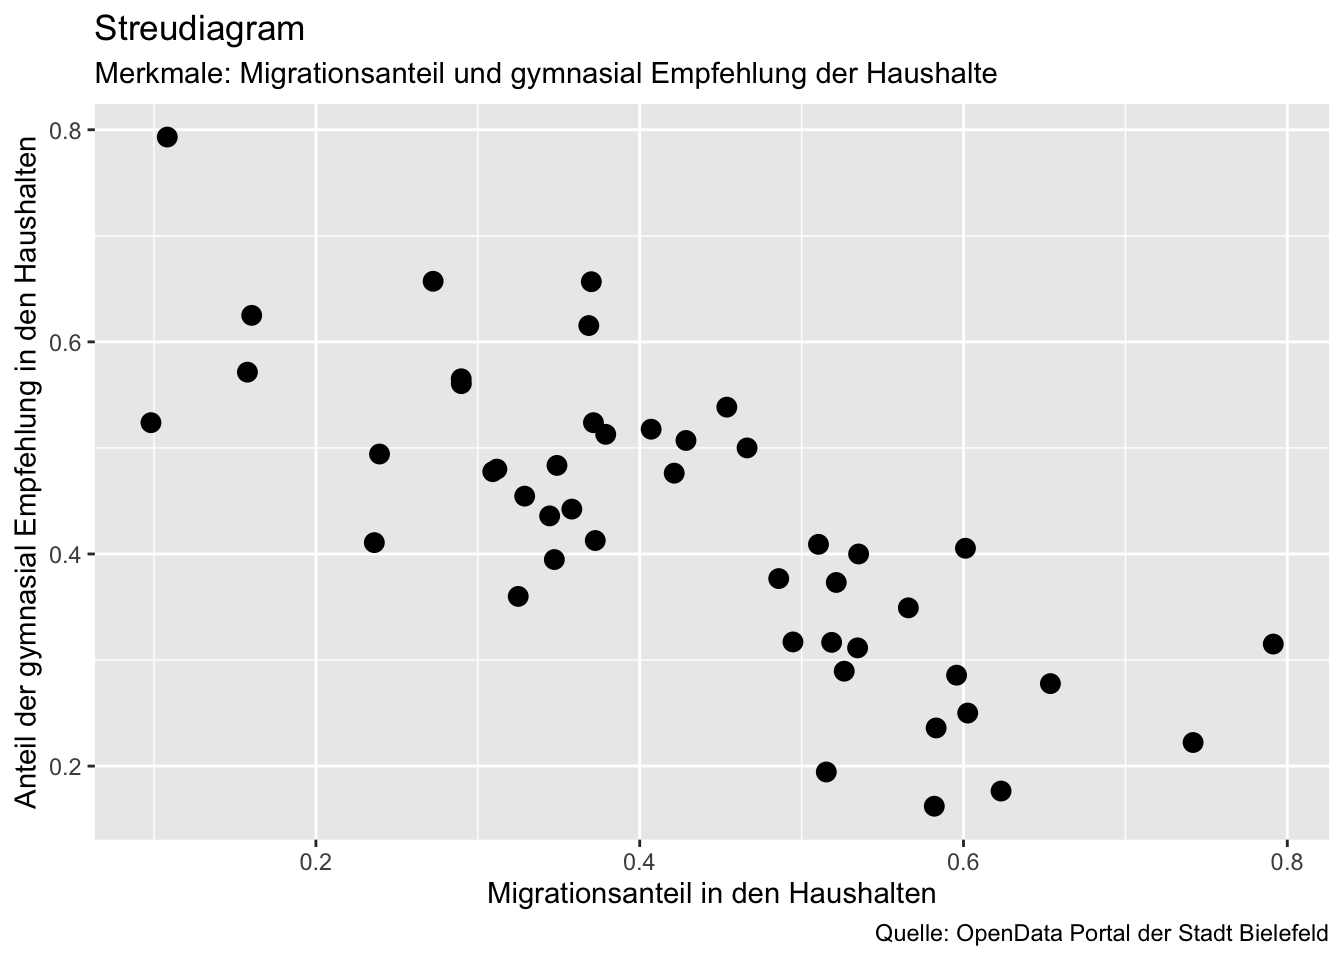
\includegraphics{Statistik_ue2_6_files/figure-latex/scatterplot-1.pdf}

\hypertarget{der-korrelationskoeffizient}{%
\subsection{Der
Korrelationskoeffizient}\label{der-korrelationskoeffizient}}

\begin{Shaded}
\begin{Highlighting}[]
\FunctionTok{cor}\NormalTok{(Belastungen}\SpecialCharTok{$}\NormalTok{Anteil\_Gym, Belastungen}\SpecialCharTok{$}\NormalTok{B\_Migration)}
\end{Highlighting}
\end{Shaded}

\begin{verbatim}
## [1] -0.7736984
\end{verbatim}

\textbf{Antwort: Der Korrelationskoeffizient betrag -0.774. Somit
befindet sich hier eine negative Korrelation mit einem mittleren bis
starken Zusammenhang.Es ist für die Daten folgendes anzunehmen. Je höher
der Migrationsanteil in den jeweiligen Haushalten ist, umso kleiner ist
der Anteil an gymnasial Empfehlungen in den dazugehörigen Haushalten.}

\hypertarget{aufgabe-7}{%
\section{Aufgabe 7}\label{aufgabe-7}}

\textbf{1. Schlechte Beispiel} Quelle:
\url{https://www.pgpf.org/sites/default/files/0070_discretionary_spending_categories-full.gif}

\begin{figure}
\centering
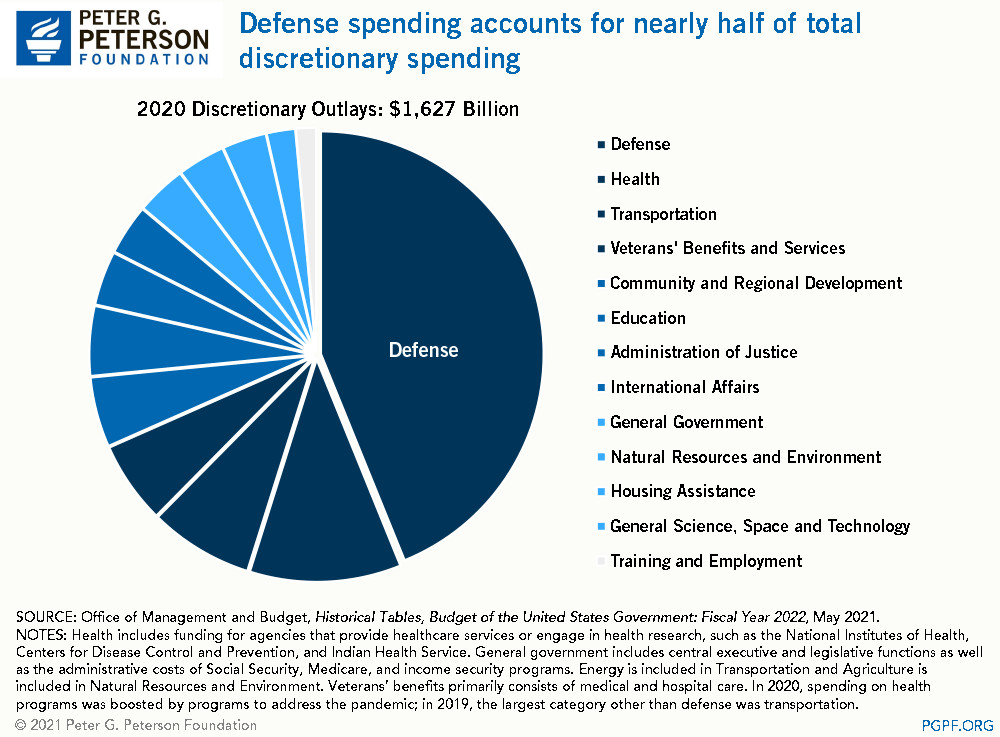
\includegraphics[width=0.7\textwidth,height=\textheight]{figures/pie-Chart_pp_foundation.gif}
\caption{Figure 1}
\end{figure}

Antwort: Unübersichtliche Farbwahl der ``Kuchenteile'', prozentuale
Anteile sind ebenfalls nicht erkennbar \textbf{2. Schlechte Beispiel}
Quelle: \url{https://i.redd.it/3ubrij7v3c081.jpg}, Hauptquelle: ARD.de

\begin{figure}
\centering
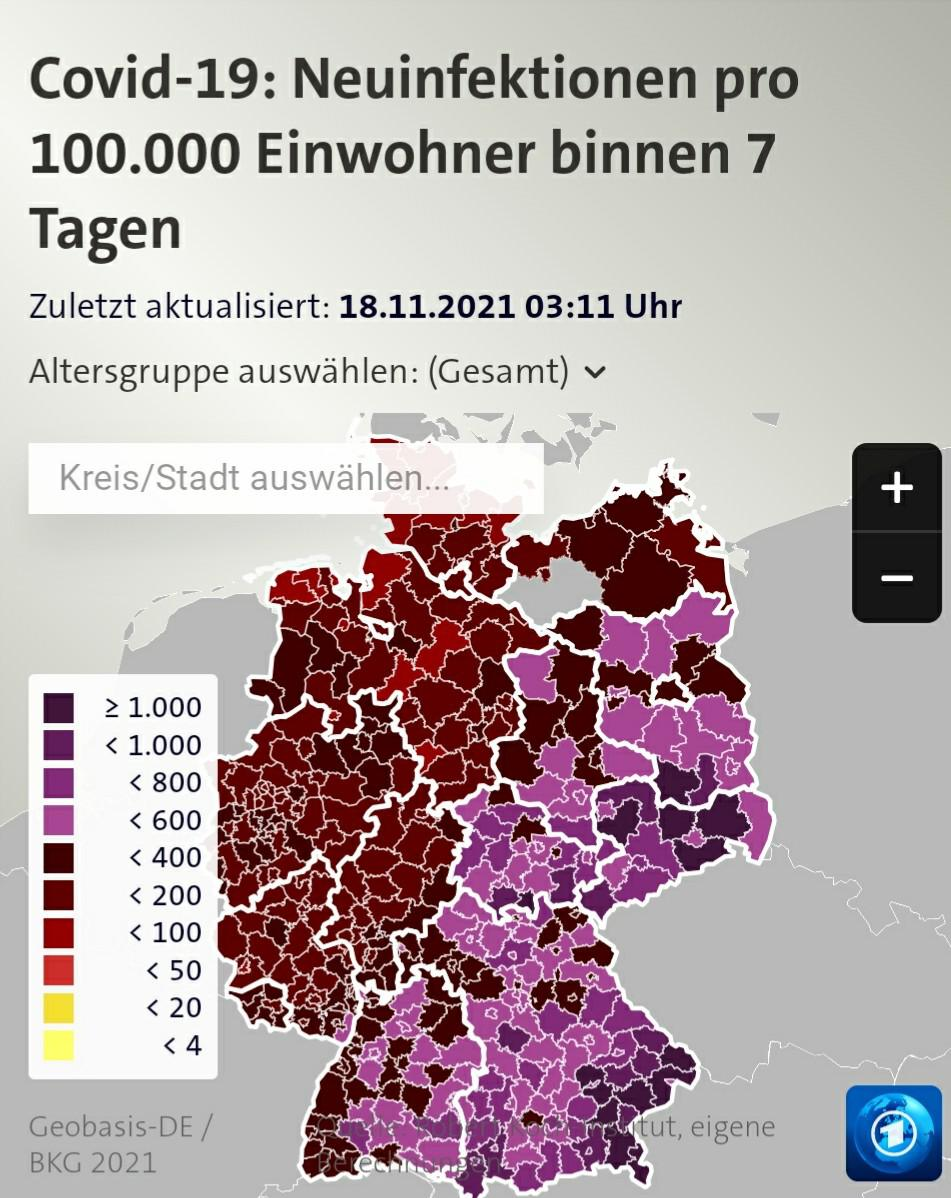
\includegraphics[width=0.7\textwidth,height=\textheight]{figures/ard_covid.jpg}
\caption{Figure 2}
\end{figure}

Antwort: In diesem Fall ist ebenfalls die Farbwahl sehr ungünstig,
insbesondere vor dem Hintergrund der Einteilung der Anzahl und der Größe
der Farbbereiche \textbf{3. Schlechte Beispiel} Quelle:
\url{https://digitalpresent.tagesspiegel.de/die-besten-erklaerstuecke-zum-coronavirus-weltweit},
Hauptquelle: Financial Times

\begin{figure}
\centering
\includegraphics[width=0.7\textwidth,height=\textheight]{figures/ft-corona.webp}
\caption{Figure 3}
\end{figure}

Antwort: An diesem Beispiel ist der Plot sehr beladen mit Informationen.
Die einzelnen Linien sind gut voneinander zu trennen.

\end{document}
